% vim: set nospell nowrap textwidth=0 wrapmargin=0 formatoptions-=t:
\RequirePackage[l2tabu,orthodox]{nag}
\documentclass[9pt]{article}
\usepackage{lmodern}
\usepackage{tikz}
\usepackage{tikz-dimline}
\usepackage{poisson}
\usetikzlibrary{hobby}
\usetikzlibrary{calc,intersections,through,backgrounds}
\usetikzlibrary{positioning, fit, arrows.meta, shapes}
\usetikzlibrary{decorations.pathreplacing, decorations.markings,decorations.pathmorphing}
% \usetikzlibrary{decorations}
\usepackage[paperwidth=17.1cm,paperheight=10.568603cm,margin=0in,heightrounded]{geometry}
\usepackage{mathabx}
\usepackage[center,pdflatex,frame]{crop}
\usetikzlibrary{circuits.ee.IEC}
\usetikzlibrary{shadings}
\usetikzlibrary{patterns}

% \usepackage{etoolbox}
% \BeforeBeginEnvironment{tabular}{\begin{center}\small}
% \AfterEndEnvironment{tabular}{\end{center}}

\definecolor{lightgrey}{rgb}{0.918,0.929,0.929}
\definecolor{stilllightergrey}{rgb}{0.959,0.9645,0.9645}
\definecolor{coolgrey}{rgb}{0.6156,0.6156,0.6156}
\definecolor{darkergrey}{rgb}{0.3078,0.3078,0.3078}
\definecolor{intermediategrey}{rgb}{0.7668,0.7723,0.7723}
\definecolor{lightblue}{rgb}{0.831,0.937,0.988}
\definecolor{lightgreen}{rgb}{0.6,0.847,0.7882}
\definecolor{imperialblue}{rgb}{0,0.243,0.455}
\definecolor{lime}{rgb}{0.7686,0.8392,0}
\definecolor{darkteal}{rgb}{0.05882,0.5098,0.5686}
\definecolor{darkgreen}{rgb}{0.00784,0.53725,0.23137}
\definecolor{orange}{rgb}{0.8235,0.25098,0}
\definecolor{lemonyellow}{rgb}{1,0.847058,0.003921}
\definecolor{poolblue}{rgb}{0.047,0.631,0.803}
\definecolor{processblue}{rgb}{0,0.52156,0.79215}
\definecolor{seaglass}{rgb}{0.215,0.623,0.623}
\definecolor{teal}{rgb}{0,0.556786,0.666}
\definecolor{imperialmoddedblue}{rgb}{0,0.43137,0.68627}
\definecolor{brick}{rgb}{0.64705,0.098039,0}
\definecolor{imperialmoddedred}{rgb}{0.8667,0.14509,0.00392}
\definecolor{imperialmoddedviolet}{rgb}{0.588235,0,0.470588}
\definecolor{iris}{rgb}{0.466667,0.145098,0.513725}
\definecolor{magentapink}{rgb}{0.784314,0.117647,0.470588}
\definecolor{raspberry}{rgb}{0.568627,0,0.282353}
\definecolor{cherry}{rgb}{0.835294,0,0.196078}
\definecolor{tangerine}{rgb}{0.92549,0.45098,0}
\definecolor{darkgreen}{rgb}{0.007843,0.537255,0.231373}
\definecolor{kermitgreen}{rgb}{0.4,0.643137,0.039216}

\setlength{\parindent}{0pt}
\setlength{\fboxsep}{0pt}%
\setlength{\fboxrule}{1pt}%
\setlength\tabcolsep{2pt}
% define layers
\pgfdeclarelayer{foreground}
\pgfdeclarelayer{background}
% tell TikZ how to stack them (back to front)
\pgfsetlayers{background,main,foreground}

\pagestyle{empty}

\tikzset{PHEV block/.style={rectangle,draw=coolgrey,thick,minimum height=20mm,minimum width=12mm,align=center,inner sep=2pt,text=black,text width=18mm }}
\tikzset{battery block/.style={PHEV block,draw=black,fill=intermediategrey,minimum height=9mm}}
\tikzset{xEV block/.style={PHEV block,draw=black}}
\tikzset{module block/.style={xEV block,draw=black,rounded corners,minimum height=8mm,font=\footnotesize,text width=10mm,inner sep=3pt}}
\tikzset{cellsinmodule block/.style={module block}}
\tikzset{ghost block/.style={PHEV block,minimum width=6mm,draw=none}}
\tikzset{differential block/.style={xEV block,minimum height=9mm,minimum width=6mm,text width=0pt,inner sep=0pt}}
\tikzset{wheel block/.style={xEV block,minimum height=4mm,minimum width=16mm,text width=0pt,inner sep=0pt}}
\tikzset{>=Stealth}
\tikzset{coupling lines/.style={black,semithick}}

\tikzset{
    pics/blob/.style={
        code={
            \draw[use Hobby shortcut, fill, closed] (0,0) +($(0:1+4*rnd)$)
            \foreach \a in {60,120,...,350} {  .. +($(\a: 1+4*rnd)$) };
        }
}}
\newcounter{mathseed}
\setcounter{mathseed}{3}

\newcommand{\flangecoupling}[2]
{
    \draw [coupling lines] (node cs:name=#1, angle= 10) to (node cs:name=#2, angle=170);
    \draw [coupling lines] (node cs:name=#1, angle=-10) to (node cs:name=#2, angle=190);
}

\newcommand{\threephasewiring}[2]
{
    \draw [coupling lines] (node cs:name=#1, angle= 20) to (node cs:name=#2, angle=160);
    \draw [coupling lines] (node cs:name=#1, angle=-20) to (node cs:name=#2, angle=200);
    \draw [coupling lines] (#1) to (#2);
}


\begin{document}
\edef\mylistpos{\poissonpointslist{2.45}{2.05}{0.07}{10}}
\edef\mylistneg{\poissonpointslist{3}{2.05}{0.08}{9}}
\begin{figure}[p]
    \begin{center}
        % \fbox{
        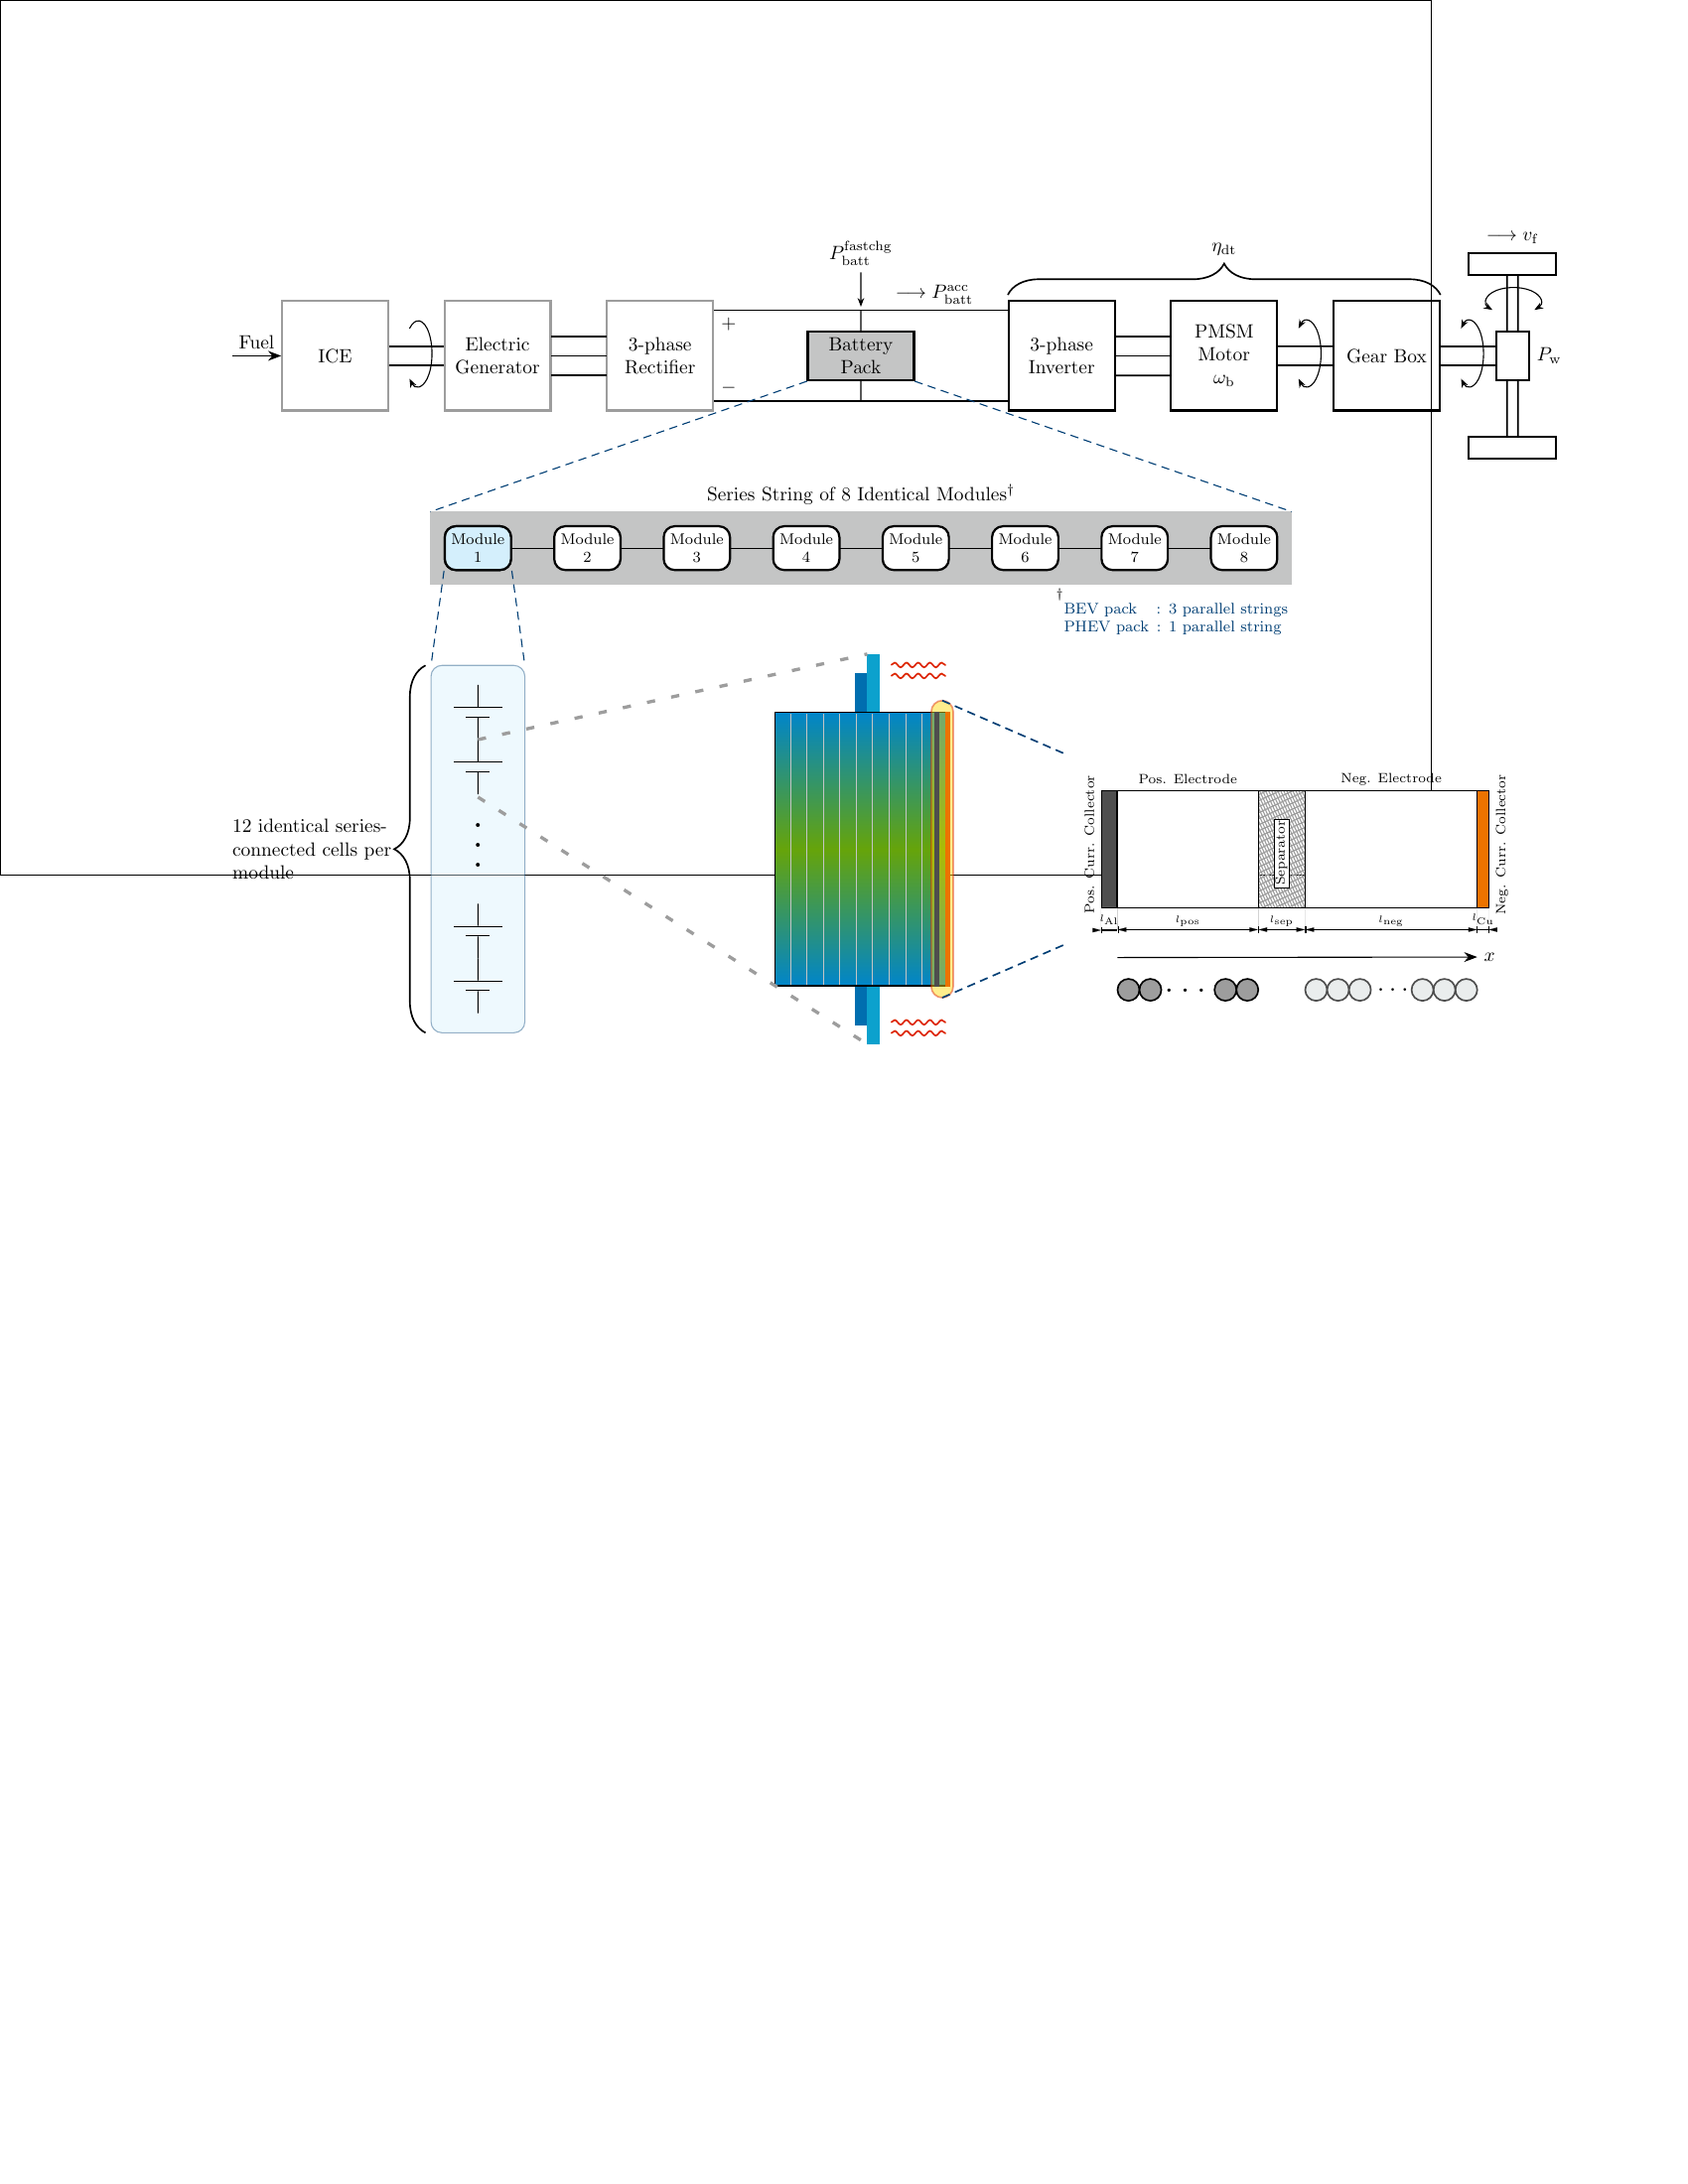
\begin{tikzpicture}[auto,scale= 0.7, every node/.append style={transform shape},circuit ee IEC]

            \node [PHEV block] (ICEngineNode) {ICE};

            \node [PHEV block]         (MGSet1Node)            [right=of ICEngineNode]     {Electric\\Generator};
            \node [PHEV block]         (RectifierNode)         [right=of MGSet1Node]       {3-phase Rectifier};
            % \node [battery block]      (BatteryNode)           [right=8mm of RectifierNode]    {Battery Pack};
            % \node [xEV block]          (InverterNode)          [right=23mm of BatteryNode]      {3-phase Inverter};
            \node [battery block]      (BatteryNode)           [right=17mm of RectifierNode]    {Battery Pack};
            \node [xEV block]          (InverterNode)          [right=17mm of BatteryNode]      {3-phase Inverter};
            \node [xEV block]          (MotorDriveNode)        [right=of InverterNode]     {PMSM Motor\\$\omega_\mathrm{b}$};
            \node [xEV block]          (TransmissionNode)      [right=of MotorDriveNode]   {Gear Box};
            \node [differential block] (DifferentialNode)      [right=of TransmissionNode] {};
            \node [ghost block]        (DifferentialNodeGhost) [right=of TransmissionNode] {};
            \node [wheel block]        (LeftWheelNode)         [above=of DifferentialNode] {};
            \node [wheel block]        (RightWheelNode)        [below=of DifferentialNode] {};

            \draw [->] ($(ICEngineNode.west) + (-9mm,0)$) to [edge label = Fuel] (ICEngineNode);
            \flangecoupling{ICEngineNode}{MGSet1Node}
            \draw [->, -{Stealth[length=1.125mm]},thin] ($(ICEngineNode.east)!0.5!(MGSet1Node.west) + (-1.25mm,5mm)$) arc [start angle=130,end angle=-130,y radius=6mm,x radius=2.5mm];
            \threephasewiring{MGSet1Node}{RectifierNode}
            \draw [name path=dcbuspos] (node cs:name=RectifierNode, angle= 40) to node [swap,pos=0.05] {$+$} (node cs:name=InverterNode, angle= 140);
            \draw [name path=dcbusneg] (node cs:name=RectifierNode, angle=-40) to node [pos=0.05] {$-$} (node cs:name=InverterNode, angle=-140);
            \path [name path=batterynorthverticalextended] (BatteryNode.north) -- +(0,10mm);
            \draw [name intersections={of=dcbuspos and batterynorthverticalextended,by={plus}}] (BatteryNode.north) -- (plus);
            \path [name path=batterysouthverticalextended] (BatteryNode.south) -- +(0,-10mm);
            \draw [name intersections={of=dcbusneg and batterysouthverticalextended,by={minus}}](BatteryNode.south) -- (minus);
            \threephasewiring{InverterNode}{MotorDriveNode}
            \flangecoupling{MotorDriveNode}{TransmissionNode}
            \draw [<->, {Stealth[length=1.125mm]}-{Stealth[length=1.125mm]},thin] ($(MotorDriveNode.east)!0.5!(TransmissionNode.west) + (-1.25mm,5mm)$) arc
                [start angle=130,end angle=-130,y radius=6mm,x radius=2.5mm];
            \flangecoupling{TransmissionNode}{DifferentialNodeGhost}
            \draw [<->, {Stealth[length=1.125mm]}-{Stealth[length=1.125mm]},thin]
                ($(TransmissionNode.east)!0.5!(DifferentialNode.west) + (-1.25mm,5mm)$)
                arc [start angle=130,end angle=-130,y radius=6mm,x radius=2.5mm];
            \draw [coupling lines] ($(LeftWheelNode.south)+(1mm,0)$) -- ($(DifferentialNode.north)+(1mm,0)$);
            \draw [coupling lines] ($(LeftWheelNode.south)+(-1mm,0)$) -- ($(DifferentialNode.north)+(-1mm,0)$);
            \draw [<->, {Stealth[length=1.125mm]}-{Stealth[length=1.125mm]},thin] ($(DifferentialNode.north)!0.5!(LeftWheelNode.south) + (4mm,-1.25mm)$)
                arc [start angle=-40,end angle=220,y radius=2.5mm,x radius=5mm];
            \draw [coupling lines] ($(RightWheelNode.north)+(1mm,0)$) -- ($(DifferentialNode.south)+(1mm,0)$);
            \draw [coupling lines] ($(RightWheelNode.north)+(-1mm,0)$) -- ($(DifferentialNode.south)+(-1mm,0)$);
            \path (plus) to node  {$\longrightarrow P^\mathrm{acc}_\mathrm{batt}$} (node cs:name=InverterNode, angle=140);
            \node (pfastchgannotation) [above=7mm of plus] {$P^\mathrm{fastchg}_\mathrm{batt}$};
            \draw [->,-{Stealth[length=1.125mm]},shorten >=0.5mm] (pfastchgannotation) -- (plus);

            \node (vfarrowandannotation) [above=1pt of LeftWheelNode.north]     {$\longrightarrow v_\mathrm{f}$};
            \node (Pwannotation)         [right=0.1mm of DifferentialNode.east] {$P_\mathrm{w}$};
            \draw [semithick,decorate,decoration={brace,raise=2pt,amplitude=4mm}] (InverterNode.north west) to node[yshift=7mm] {$\eta_\mathrm{dt}$} (TransmissionNode.north east);


            \foreach \modulecount in {0,...,7}
            \node [fill=white,module block,below=25mm of MotorDriveNode.south east,anchor=east,xshift=\modulecount*-20mm] (loopmodule\modulecount) {Module \pgfmathparse{int(8-\modulecount)} \pgfmathresult};

            \begin{scope}[on background layer]
                \node [fill=intermediategrey,label={Series String of 8 Identical Modules$^\dag$},fit=(loopmodule0)(loopmodule1)(loopmodule2)(loopmodule3)(loopmodule4)(loopmodule5)(loopmodule6)(loopmodule7),transform shape=false,inner sep=5pt,outer sep=0pt] (modulefitnode) {};

                % \node [below= of modulefitnode.east,anchor=east,inner sep=0pt,outer sep=0pt,yshift=1mm] (daggernotation) {$^\dag$};
                % \node [right=12.5mm of daggernotation,text=imperialblue,font=\footnotesize,inner sep=0pt,outer sep=0pt,label={[label distance=-3mm]176:$^\dag$}] (BEVstringannotation)
                % \node [right=-1pt of daggernotation,text=imperialblue,font=\footnotesize,inner sep=0pt,outer sep=0pt,yshift=-6pt] (BEVstringannotation)
                \node [below= of modulefitnode.south east,text=imperialblue,font=\footnotesize,inner sep=0pt,outer sep=0pt,anchor=north east,yshift=7mm,label={[label distance=-2mm]176.5:$^\dag$}] (BEVstringannotation)
                {
                    \begin{tabular}{lll}
                        BEV pack & : & 3 parallel strings\\
                        PHEV pack& : & 1 parallel string\\
                    \end{tabular}
                };

                \foreach \modulecount in {0,...,1}
                % \draw (loopmodule\modulecount) to node (loopmodule\pgfmathparse{int(1+\modulecount)}\pgfmathresult);
                \draw (loopmodule\modulecount) -- (loopmodule7);
            \end{scope}

            \draw [densely dashed,imperialblue] (BatteryNode.south west) -- (modulefitnode.north west);
            \draw [densely dashed,imperialblue] (BatteryNode.south east) -- (modulefitnode.north east);

            \draw ($(loopmodule7)+(0,-25  mm )$) to      [ battery={name=posterminal}] ($(loopmodule7)+(0,-35                      mm )$);
            \draw ($(loopmodule7)+(0,-35  mm )$) to      [ battery] ($(loopmodule7)+(0,-45                                         mm )$);
            \path ($(loopmodule7)+(0,-45  mm )$) -- node [ auto=false,midway,rotate=-90]{\Huge{\dots}} ($(loopmodule7)+(0,-65 mm )$);
            \draw ($(loopmodule7)+(0,-65 mm )$) to       [ battery] ($(loopmodule7)+(0,-75                                        mm )$); \draw ($(loopmodule7)+(0,-75 mm )$) to       [ battery={name=negterminal}] ($(loopmodule7)+(0,-85                     mm )$);

            \begin{scope}[on background layer]
                \node [outer sep=0pt,draw=imperialblue,rounded corners,fit=(posterminal)(negterminal),transform shape=false,fill=lightblue,opacity=0.4,inner sep=2pt,minimum height=47mm,minimum width=12mm] (cellsinmodule) {};
            \end{scope}
            \draw [semithick,decorate,decoration={brace,raise=2pt,amplitude=4mm},xshift=0pt,yshift=0pt] (cellsinmodule.south west) to node[rotate=0,yshift=0mm,xshift=-5mm, text width=30mm] {12 identical series-connected cells per module} (cellsinmodule.north west);

            \draw [densely dashed,imperialblue] (loopmodule7.south west) -- (cellsinmodule.north west);
            \draw [densely dashed,imperialblue] (loopmodule7.south east) -- (cellsinmodule.north east);

            \begin{scope}
                \path let \p1 = (loopmodule7) in node [fill=lightblue,module block] at (\x1,\y1) {Module 1};
            \end{scope}


            \begin{scope}[on background layer]
                % \node [minimum width=22mm,inner sep=0pt,minimum height=35mm,transform shape=false,draw,semithick,shading=axis, top color=processblue,bottom color=processblue,middle color=lemonyellow] (layerschematicNode) at (BatteryNode |- cellsinmodule) {};
                % \node [minimum width=22mm,inner sep=0pt,minimum height=35mm,transform shape=false,draw,semithick,shading=axis, top color=processblue,bottom color=processblue,middle color=lightblue] (layerschematicNode) at (BatteryNode |- cellsinmodule) {};
                % \node [minimum width=22mm,inner sep=0pt,minimum height=35mm,transform shape=false,draw,semithick,shading=axis, top color=kermitgreen,bottom color=kermitgreen,middle color=lemonyellow] (layerschematicNode) at (BatteryNode |- cellsinmodule) {};
                % \node [minimum width=22mm,inner sep=0pt,minimum height=35mm,transform shape=false,draw,semithick,shading=axis, top color=kermitgreen,bottom color=kermitgreen,middle color=lime] (layerschematicNode) at (BatteryNode |- cellsinmodule) {};
                \node [minimum width=22mm,inner sep=0pt,minimum height=35mm,transform shape=false,draw,semithick,shading=axis, top color=processblue,bottom color=processblue,middle color=kermitgreen] (layerschematicNode) at (BatteryNode |- cellsinmodule) {};
                % \draw [xstep=2mm,ystep=75mm,very thin,coolgrey,transform shape=false] (layerschematicNode.north east) grid (layerschematicNode.south west);
            \end{scope}

            \foreach \layerlines in {1,...,10}
            \draw [intermediategrey,very thin]  ($(layerschematicNode.south west) + (\layerlines*3mm,1pt)$) --  ($(layerschematicNode.north west) + (\layerlines*3mm,-1pt)$);

            \node [minimum height=7mm,fill=imperialmoddedblue,semithick,anchor=south,outer sep=0pt,minimum width=2mm] at (layerschematicNode.north) (cellnorthend) {};
            \node [minimum height=10.5mm,fill=poolblue,semithick,anchor=south west,outer sep=0pt,minimum width=2mm] at (cellnorthend.south east) (cellnorthendcoolingplate) {};
            \node [minimum height=7mm,fill=imperialmoddedblue,semithick,anchor=north,outer sep=0pt,minimum width=2mm] at (layerschematicNode.south) (cellsouthend) {};
            \node [minimum height=10.5mm,fill=poolblue,semithick,anchor=north west,outer sep=0pt,minimum width=2mm] at (cellsouthend.north east) (cellsouthendcoolingplate) {};

            \foreach \evaporationlines in {1,...,2}
            {
                \draw [imperialmoddedred,semithick,decorate,decoration={snake,amplitude=.3mm,segment length=1.5mm, post length=0mm}]  ($(cellnorthendcoolingplate.north east) + (2mm,\evaporationlines*-2mm)$) -- ($(cellnorthendcoolingplate.north east) + (12mm,\evaporationlines*-2mm)$);
                \draw [imperialmoddedred,semithick,decorate,decoration={snake,amplitude=.3mm,segment length=1.5mm, post length=0mm}]  ($(cellsouthendcoolingplate.south east) + (2mm,\evaporationlines*2mm)$) -- ($(cellsouthendcoolingplate.south east) + (12mm,\evaporationlines*2mm)$);
            }

            % \draw ($(loopmodule7)+(0,-30  mm )$) to      [ battery] ($(loopmodule7)+(0,-40                                         mm )$);
            \draw [very thick,loosely dashed,coolgrey] ($(loopmodule7)+(0,-35  mm )$) -- (cellnorthendcoolingplate.north west);
            \draw [very thick,loosely dashed,coolgrey] ($(loopmodule7)+(0,-45.5  mm )$) -- (cellsouthendcoolingplate.south west);

            % \draw [ultra thick] (layerschematicNode.south east) rectangle ($(layerschematicNode.north east) + (-2mm,0)$);
            \draw [ultra thick,darkergrey] ($(layerschematicNode.south east) + (-2mm,0)$) -- ($(layerschematicNode.north east) + (-2mm,0)$);
            \draw [ultra thick,tangerine] (layerschematicNode.south east) -- (layerschematicNode.north east);

            \begin{scope}[on background layer]
                \draw [semithick,fill=lemonyellow,draw=imperialmoddedred,opacity=0.45,rounded corners] ($(layerschematicNode.south east) + (1mm,-2mm)$) rectangle ($(layerschematicNode.north east) + (-3mm,2mm)$);
            \end{scope}

            \node [label={[yshift=-10mm,rotate=90,text depth=1ex] \scriptsize Pos. Curr. Collector},thin,minimum height=15mm,draw,fill=darkergrey,transform shape=false,anchor=west,minimum width=2mm,inner sep=0pt] at (loopmodule1.west |- layerschematicNode) (poscc) {};
            % \dimline{(poscc.south west)}{(poscc.south east)}{$L_\mathrm{Al}$}
            % \dimline[line style={arrows=dimline reverse-},label style={fill=none,above=0.1mm,inner sep=0pt},extension start length=2mm, extension end length=2mm]{($(poscc.north west)+ (0,2mm)$)}{($(poscc.north east)+ (0,2mm)$)}{$\scriptscriptstyle L_\mathrm{Al}$}
            \dimline[line style={arrows=dimline reverse-},label style={fill=none,above=0.9mm,inner sep=0pt},extension start length=-4mm, extension end length=-4mm]{($(poscc.south west)+ (0,-4mm)$)}{($(poscc.south east)+ (0,-4mm)$)}{$\scriptscriptstyle l_\mathrm{Al}$}
            % \draw [->,shorten >=1pt] ($(layerschematicNode.north east) + (-2mm,1pt)$) to [in=90,bend left = 45] (poscc.north);

            \node [label={above:\scriptsize Pos. Electrode},thin,minimum height=15mm,draw,fill=white,minimum width=18mm,outer sep=0pt,anchor=west,transform shape=false] at (poscc.east) (posdomain) {};
            % \dimline[extension start style={ultra thin,densely dash dot},label style={fill=none,above=0.1mm,inner sep=0pt},extension start length=-3mm, extension end length=-3mm]{($(posdomain.south west)+ (0,-3mm)$)}{($(posdomain.south east)+ (0,-3mm)$)}{$\scriptscriptstyle L_\mathrm{pos}$}
            \dimline[label style={fill=none,above=0.5mm,inner sep=0pt},extension start length=-4mm, extension end length=-4mm]{($(posdomain.south west)+ (0,-4mm)$)}{($(posdomain.south east)+ (0,-4mm)$)}{$\scriptscriptstyle l_\mathrm{pos}$}

            \begin{pgfonlayer}{foreground}
                \node [label={[fill=white,rotate=90,yshift=1.5mm,xshift=10mm,inner sep=1pt,draw,ultra thin]below:\scriptsize Separator},thin,minimum height=15mm,draw,minimum width=6mm,outer sep=0pt,anchor=west,transform shape=false] at (posdomain.east) (separatordomain) {};
            \end{pgfonlayer}
            \dimline[label style={fill=none,above=0.5mm,inner sep=0pt},extension start length=-4mm, extension end length=-4mm]{($(separatordomain.south west)+ (0,-4mm)$)}{($(separatordomain.south east)+ (0,-4mm)$)}{$\scriptscriptstyle l_\mathrm{sep}$}

            \begin{scope}
                \clip (separatordomain.south west) rectangle (separatordomain.north east);
                \draw [xstep=0.5mm,ystep=1mm,coolgrey,rotate=25] ($(separatordomain.south)+(-10mm,-10mm)$) grid ($(separatordomain.north)+(10mm,10mm)$);
            \end{scope}
            \node [label={[yshift=-1pt]above:\scriptsize Neg. Electrode},thin,minimum height=15mm,draw,minimum width=22mm,outer sep=0pt,anchor=west,transform shape=false,fill=white] at (separatordomain.east) (negdomain) {};
            \dimline[label style={fill=none,above=0.5mm,inner sep=0pt},extension start length=-4mm, extension end length=-4mm]{($(negdomain.south west)+ (0,-4mm)$)}{($(negdomain.south east)+ (0,-4mm)$)}{$\scriptscriptstyle l_\mathrm{neg}$}
            \node [label={[fill=none,rotate=90,yshift=-2.0mm,xshift=11.5mm,inner sep=1pt,ultra thin]below:\scriptsize Neg. Curr. Collector},thin,minimum height=15mm,draw,minimum width=1.5mm,outer sep=0pt,anchor=west,transform shape=false,fill=tangerine,inner sep=0pt] at (negdomain.east) (negcc) {};
            \dimline[line style={arrows=-dimline reverse},label style={fill=none,above=0.9mm,inner sep=0pt},extension start length=-4mm, extension end length=-4mm]{($(negcc.south west)+ (0,-4mm)$)}{($(negcc.south east)+ (0,-4mm)$)}{$\scriptscriptstyle l_\mathrm{Cu}$}

            \begin{scope}[on background layer]
                \node[thick,fit=(poscc)(negcc),draw=imperialmoddedred,fill=lemonyellow,opacity=0, transform shape=false,rounded corners,inner sep=4.5mm] (layerbackgroundnode) {};
            \end{scope}

            \draw [semithick,densely dashed,imperialblue] ($(layerschematicNode.north east) + (-1.0mm,2mm)$) -- (layerbackgroundnode.north west);
            \draw [semithick,densely dashed,imperialblue] ($(layerschematicNode.south east) + (-1.0mm,-2mm)$) -- (layerbackgroundnode.south west);
            \draw [->,thin] ($(poscc.south east)+(0,-9mm)$) -- node[pos=1.0,right] {$x$} ($(negcc.south west)+(0,-9mm)$);

            \foreach \possphericalparticle in {0,...,1}
            \draw [fill=coolgrey,semithick] ($(posdomain.south west) + (2mm+\possphericalparticle*4mm,-15mm)$) circle [radius=2mm] ($(posdomain.south east) + (-2mm-\possphericalparticle*4mm,-15mm)$) circle [radius=-2mm];
            \foreach \negsphericalparticle in {0,...,2}
            \draw [fill=lightgrey,draw=darkergrey,very thin,semithick] ($(negdomain.south west) + (2mm+\negsphericalparticle*4mm,-15mm)$) circle [radius=2mm] ($(negdomain.south east) + (-2mm-\negsphericalparticle*4mm,-15mm)$) circle [radius=-2mm];
            \node at ($(poscc.south west) + (16mm,-15mm)$) {\huge{\dots}};
            \node at ($(negcc.south west) + (-15mm,-15mm)$) {\Large{\dots}};

            \begin{scope}
                \clip (posdomain.south west) rectangle (posdomain.north east);
                \foreach \x/\y in \mylistpos{
                    \pgfmathsetmacro{\scale}{0.01+0.01*rnd}
                    \pic at ($(posdomain.south west)+(\x+.06,\y+.05)$)
                    [line width=0.05mm,fill=coolgrey,
                    scale=\scale, rotate=360*rnd]{blob};
                }
            \end{scope}

            \begin{scope}
                \clip ($(negdomain.south west)+(1pt,1pt)$) rectangle ($(negdomain.north east)+(-1pt,-1pt)$);
                \foreach \x/\y in \mylistneg {
                    \pgfmathsetmacro{\scale}{0.011+0.011*rnd}
                    \pic at ($(negdomain.south west)+(\x+.05,\y+.04)$)
                    [line width=0.05mm,fill=lightgrey,
                    scale=\scale, rotate=359*rnd]{blob};
                }
            \end{scope}

        \end{tikzpicture}
        % }
    \end{center}
\end{figure}

\end{document}
